\documentclass[12pt,letterpaper]{article}

% Image support with PDF conversion
\usepackage[pdftex]{graphicx}
% Inserts a line feed between paragraphs, because it makes me feel grown up
\usepackage{parskip}
% Underline text using \uline{...}
\usepackage[normalem]{ulem}
% Sane URL handling
\usepackage{url}
% Math equations
\usepackage{mathtools}
% source code typesetting
\usepackage{algpseudocode}
\usepackage{listings}
% Implement the ARRL's oddly specific margin and page number equirements
\usepackage[top=0.8in, bottom=1in, left=0.75in, right=0.75in]{geometry}
\pagenumbering{gobble}


\title{Clarifying Amateur Bell 202}

\author{Kenneth Finnegan, W6KWF\\
\small Masters Student, Electrical Engineering Department\\
\small California Polytechnic State University, San Luis Obispo\\
\small \texttt{http://blog.thelifeofkenneth.com/}\\
\small \texttt{kennethfinnegan2007@gmail.com}\\
\and
Bridget Benson, Ph.D.\\
\small Assistant Professor, Electrical Engineering Department\\
\small California Polytechnic State University, San Luis Obispo\\
\small \texttt{http://www.calpoly.edu/~bbenson/}\\
\small \texttt{bbenson@calpoly.edu}}


\begin{document}
\maketitle

\begin{abstract}
	Since its inception more than three decades ago, 
	packet radio has seen several huge changes in technology
	and applications. 
	Despite its age, the 1200 baud Bell 202 modulation used in some
	of the earliest packet systems still enjoys a wide user base
	in several of the major packet networks still in operation.
	Oddly, despite being one of the longest-lived amateur packet modulations in use,
	the amateur community seems to have failed to ever write a detailed
	specification document for this integral part of so many packet systems.
	This paper curates the information garnered from countless sources
	in the hopes that other amateurs developing modems for 
	this prototypical modulation
	don't need to follow the author in spending such an inordinate amount of
	time and energy researching and reverse-engineering what should be a
	well-established specification.
	
	
	\textbf{Keywords:} AFSK, AX.25, Bell 202, Packet Radio, Specification
\end{abstract}


\section{Bell 202 in Amateur Radio}
\label{sec:bell202history}

Bell 202 is an audio frequency shift keyed (AFSK) modulation that
encodes data by shifting between 1200Hz and 2200Hz tones.
These tones represent a binary one or zero respectively and transitions happen
at a rate of 1200 symbols per second.
Originally developed by AT\&T for use on the telephone network \cite{202tspec},
Bell 202 was selected for amateur radio packet operations due to the abundance
of modems available on the second-hand market in 1981 when the FCC authorized
amateur packet operations \cite{gatewaypacket}.

\begin{figure}
	\centering
	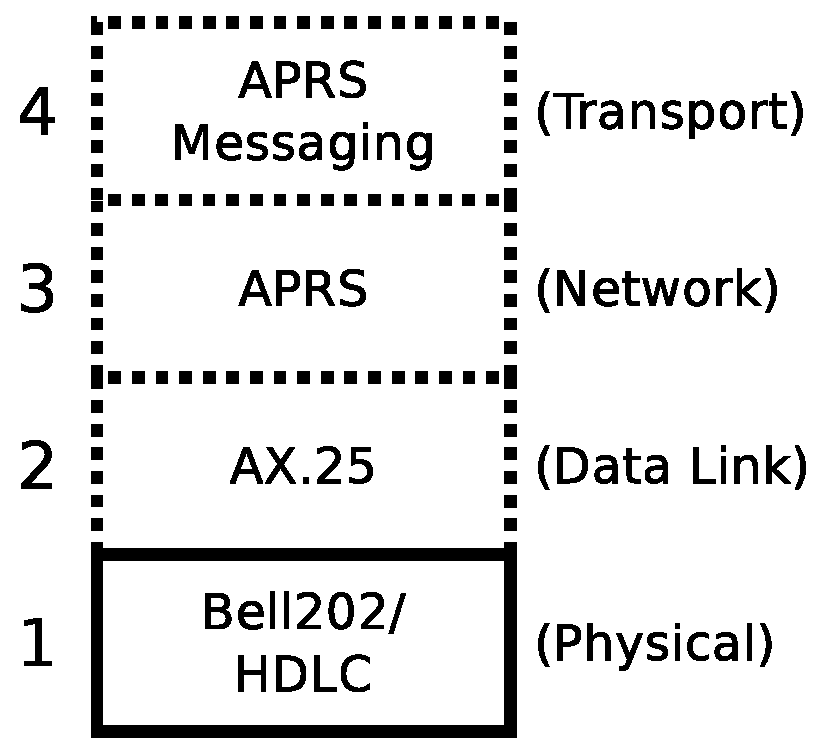
\includegraphics[width=0.4\textwidth]{src/dia/osi_bell202}
	\caption{OSI network layers for a typical packet radio application}
	\label{fig:osibell}
\end{figure}

Like most real-world network protocols, there isn't a particularly clean
mapping of packet radio protocols to the seven layers of the OSI
network model. To help clarify references to the different layers in this article,
figure \ref{osibell} shows Bell 202 in the context of its application
to APRS.
Due to Amateur radio operators
using Bell 202 as a physical layer below AX.25, which is a derivative of
X.25, it implicitly includes the High-Level Data Link Control (HDLC) 
protocol for framing and bit stuffing in the layer 1 protocol \cite{n1vgphy}.
This means that the original 1200Hz mark and 2200Hz space symbols
do not directly represent one and zero.
The AX.25 data stream is encoded using the 
inverted non-return to zero (NRZI) encoding,
which requires zeros in the original bit stream to be encoded as a change
between 1200Hz and 2200Hz and ones to be encoded as transmitting the same
tone during two consecutive symbol periods \cite{iso13239}.

\section{Bell 202 Transmission Format}

\begin{figure}
	\centering
	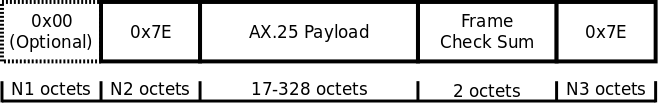
\includegraphics[width=1.0\textwidth]{src/dia/bell202}
	\caption{Bell 202/HDLC frame format}
	\label{fig:bell202format}
\end{figure}

Figure \ref{fig:bell202format} shows the format of a typical single frame
Bell 202 transmission. There are a number of things to
note:
\begin{itemize}
	\item The leading 0x00 octets are mentioned in very few documents
		discussing Bell 202, yet they reportedly improve modem
		throughput \cite{millerinterview}\cite{aprsunveiled}. 
		0x00 encoded in NRZI causes a symbol transition
		every clock cycle and thus provides a more effective clock 
		syncronization target than the specified 0x7E octets. 0x7E is actually 
		the longest allowable string of 1s in the frame and 
		therefore has the lowest amount of energy at the clocking frequency,
		which causes it to be the worst 
		octet for asynchronous clock recovery.
	\item The octet 0x7E is used to indicate the beginning and end of 
		Bell 202 / HDLC frames.
		There is little guidance on the numer of flag octets before
		or after frames (represented by N2 and N3 in 
		figure \ref{fig:bell202format})
		beyond stating that there must be at least one of each. The sum of
		N1 and N2 is variable in most modems via the ``TXDelay" parameter,
		which specifies how long the premble is in 10ms increments.
	\item It is permissible to encode multiple 
		frames per transmission, yet there is no guidance as to how
		many octets of 0x7E be included between them.
		Most modems insert several 0x7E octets between 
		frames.\footnote{For a specific example, the Argent Data OT3m TNC 
			with firmware r56474 inserts 3 flags before
		a frame, 7 flags between two frames, and 5 flags after the final frame.}
		Tests indicate that the number of flags between frames 
		impact throughput of the following frame, yet
		quantitative measurements of this effect proved elusive.
	\item The frame payload and frame check sum must be bit stuffed such 
		that no string of more than five 1's appear in a row.
		This is done by ``bit-stuffing" the transmitted bitsteam by
		appending a zero after any string of five ones at the transmitter,
		and subsequently dropping this zero following five ones at the 
		receiver.\footnote{Six ones in a row represent a 0x7E flag indicating 
			the end of a frame or an idle carrier.
			Seven or more ones in a row indicate an invalid channel state
			that shouldn't happen, but regularly does, so modems must be 
			able to handle arbitrary strings of ones gracefully.}
	\item Every octet is encoded and transmitted least significant bit first,
		except for the CRC-16-CCITT Frame Check Sum, 
		which is transmitted big-endian
		and most significant big first.
		\cite{n1vgphy},\cite[\S8.1.1-2]{ituv42},\cite[\S3.8]{ax25spec}.
		See section \ref{calcfcs} for further discussion.
	\item The minimum and maximum payload sizes indicated in figure 
		\ref{fig:bell202format} aren't enforced by any properties of 
		Bell 202 or HDLC, but from the Maximum Transmission Unit (MTU)
		specified in the AX.25 network stack.
		Larger frames are possible, and were often used in specialized 
		AX.25 and IPv4 packet networks \cite{pattersoninterview}.

\end{itemize}

\subsection{Excluding HDLC from AX.25 layer 2}

It is important to note that the presentation of the HDCL framing
and checksum
in figure \ref{fig:bell202format} as part of the layer 1 modulation 
instead of as part of the layer 2 AX.25 frame is 
novel to this work and hasn't been seen in any of the existing literature.
This change was made because including the frame checksum and flags
in the layer 2 documentation confuses the seperation between Bell 202 
and AX.25. 

This is particularly important when AX.25 packets are transfers across 
other layer 1 links with their own framing protocols.
The KISS serial link between a host system and modem is the most notable
transport where these fields are not included and post-facto generated by the
Bell 202 modem during transmission.
M. Chepponis and P. Karn made the technically correct decision of excluding 
HDCL framing from the binary payload transfered over KISS, but this caused
an unfortunate situation where KISS is transporting an entirely
undocumented fragment of the AX.25 packet. Figure \ref{fig:ax25format} 
shows what the AX.25 layer 2 should be presented as.

\begin{figure}
	\centering
	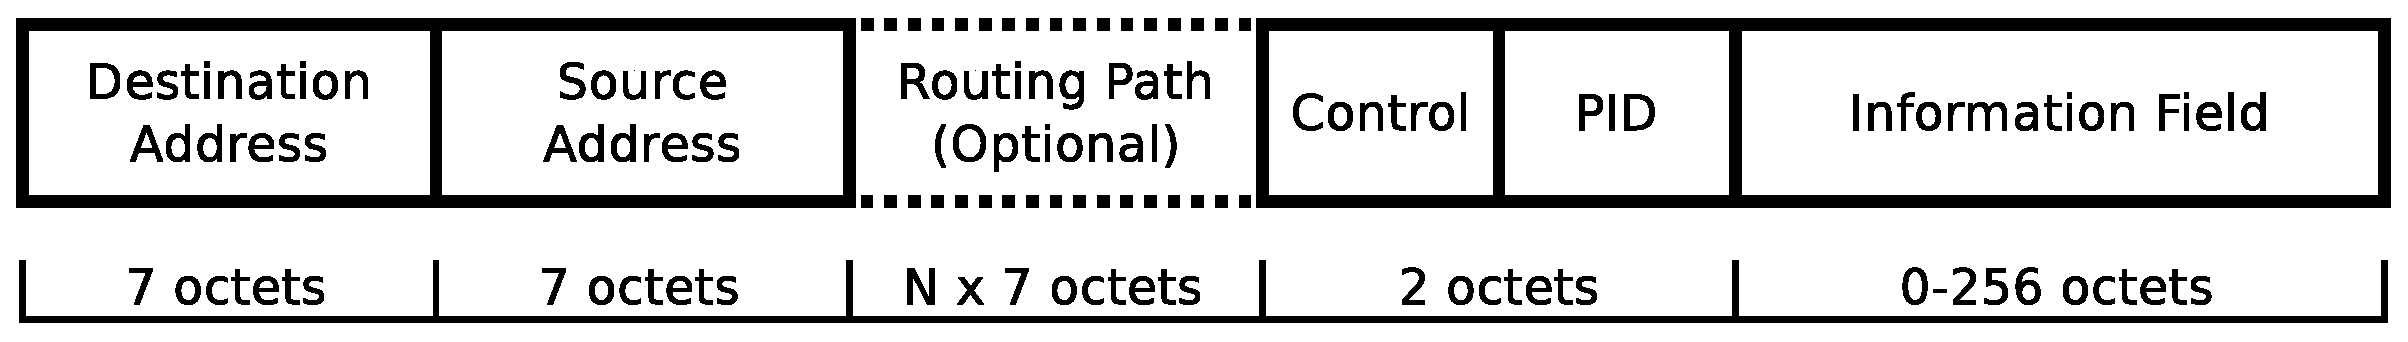
\includegraphics[width=1.0\textwidth]{src/dia/ax25}
	\caption{Modified AX.25 packet format excluding HDLC fields.}
	\label{fig:ax25format}
\end{figure}

\subsection{Calculating the Frame Check Sum}
\label{calcfcs}


The CRC used for error detection is the well-known CRC-16-CCITT which
enjoys a wide deployment in network protocols and 
systems\footnote{Example systems include HDLC, Bluetooth, the XMODEM file 
transfer protocol, and SD cards}.
Unfortunately, the language used in \S4.2.5 of the ISO specification for
HDLC \cite{iso13239} is particularly awkward, 
and doesn't lend itself well to implementation.
For the sake of clarity, figure \ref{fig:crcccittcode} 
presents one possible algorithm to
calculate the CRC checksum of a complete frame.
The constant 0x8408 comes from a bit reversal of the 0x1021 generator polynomial
since the presented algorithm calculates the CRC in bit reversed order.

The order of the two octets and bit order of the checksum 
as transmitted over the air 
is particularly muddled in the existing amateur literature, 
since most amateur sources call for sending the
checksum little-endian, while ITU V.42 \S8.1.2.3 specifies big-endian,
as is the convention for most network protocols.
It's theorized that this confusion comes from the fact that most amateurs are copying
available reference implementations of the CRC checksum that,
unbeknownst to the amateur, already integrate the ones completement,
bit reversal, and conversion from little-endian to network order of the CRC.


\begin{figure}
	\begin{algorithmic}[1]
		\Function{calculate\_crc}{$frame[~], frame\_length$}
		\State $crc \gets \texttt{0xFFFF}$

		\ForAll{$byte \gets frame_{0}, frame_{frame\_length-1}$}
		\ForAll {$bit \gets byte_{LSb}, byte_{MSb}$}
		\If {$crc_{LSb} \neq bit$}
			\State $crc \gets (crc \gg 1) \textrm{ XOR } \texttt{0x8408}$
			%\Comment{Right shift and XOR with bit-reversed polynomial}
		\Else
			\State $crc \gets crc \gg 1$
			%\Comment{Only right shift}
		\EndIf
		\EndFor
		\EndFor

		\State $crc \gets crc \textrm{ XOR } \texttt{0xFFFF}$
		%\Comment{Take one's complement per ITU-T V.42 \S8.1.1.6.2}
		\State $crc \gets ((crc \ll 8) \textrm{ AND } \texttt{0xFF00}) + ((crc \gg 8) \textrm{ AND } \texttt{0x00FF})$

		%\Comment{Swap high and low bytes so crc is in host endian order}
		\State \textbf{return} $crc$
		\EndFunction
	\end{algorithmic}

	\caption{Algorithm to calculate CRC-16-CCITT in host-endian reverse-bit order}
	\label{fig:crcccittcode}
\end{figure}

\section{FM Deviation and Emphasis}

Once the HDLC frame is generated, encoded using NRZI, and converted into
a baseband AFSK signal, it still needs to be converted into a VHF FM signal
and transmitted to other stations. 
Since Bell 202 was originally designed for telephone loop service, 
the existing specifications give absolutely no guidance on the unique 
aspects of the amateur VHF FM physical layer, such as what 
FM deviation to target when setting modem audio levels.

While quantitatively justifying this figure is beyond the ability of the
author, a proposed specification for FM deviation is 3.5kHz for both
1200Hz and 2200Hz tones\cite{millerinterview}.

This proposal is complicated by two major issues: 
\begin{itemize}
	\item The lack of availability of the necessary 
		test equipment to measure FM deviation.
	\item The inconsistency in pre-emphasis and de-emphasis filters
		used by individual network nodes.
\end{itemize}

The VHF service monitor needed to properly set modem deviation is prohibitively
expensive for the typical packet radio operator, so presenting a figure 
such as 3.5kHz deviation to most users makes little difference.
Qualitative and home-brew solutions have been developed
for setting deviation levels\cite{n8urdev},
and these techniques should be better promoted until 
deviation meters become a standard part of a packet operator's toolkit. 

\begin{figure}
	\centering
	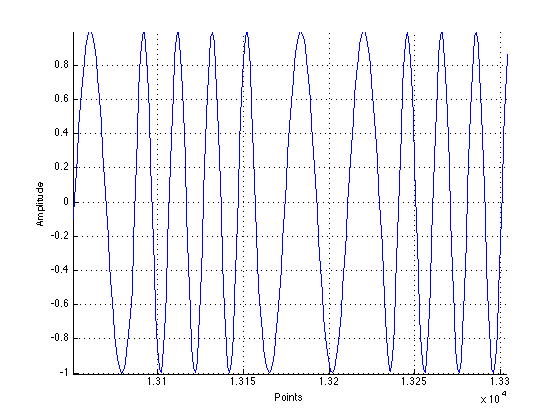
\includegraphics[width=0.7\textwidth]{src/bell202sample}
	\caption{Typical Bell 202 baseband signal}
	\label{fig:bell202sample}
\end{figure}

Pre-emphasis and de-emphasis is a concept in FM voice communications where
higher baseband frequencies are more widely modulated than lower ones
to provide a consistent signal to noise ratio.
Unfortunately, the advantage of these audio filters to packet operation 
are debatable, and they are not applied consistently. A given packet 
station is likely to have any permutation of pre-emphasised or flat 
transmit audio and de-emphasised or flat receive audio.
This means that even when one station deliberately uses flat audio,
there is no guarantee that it won't suffer from receiving another
station's pre-emphasised signal or be received by another station using de-emphasis.

Different types of Bell 202 modems vary in how sensitive they are to this high/low
pass filtering effect, but more importantly there is no benchmark established
for what level of pre-/de-emphasis a modem should tolerate.
One suitable source for such a benchmark would be to go back to the
telephone networks where Bell 202 was originally used.
Figure \ref{fig:3002} shows the allowable audio distortion of a basic type 3002
channel as used in the telephone network. Any level of distortion that falls 
inside the shaded region relative to a test tone at 1004 Hz is considered acceptable.

For application to amateur Bell 202, the distortion figures normalized to 1004Hz is 
less critical than the fact that the allowable distortion between the two
tones of interest (1200Hz and 2200Hz) is 10dB in either direction.
A valuable measurement for Bell 202 modem designers would be testing how
quickly their modem's performance falls off as it approaches these limits.

\begin{figure}
	\centering
	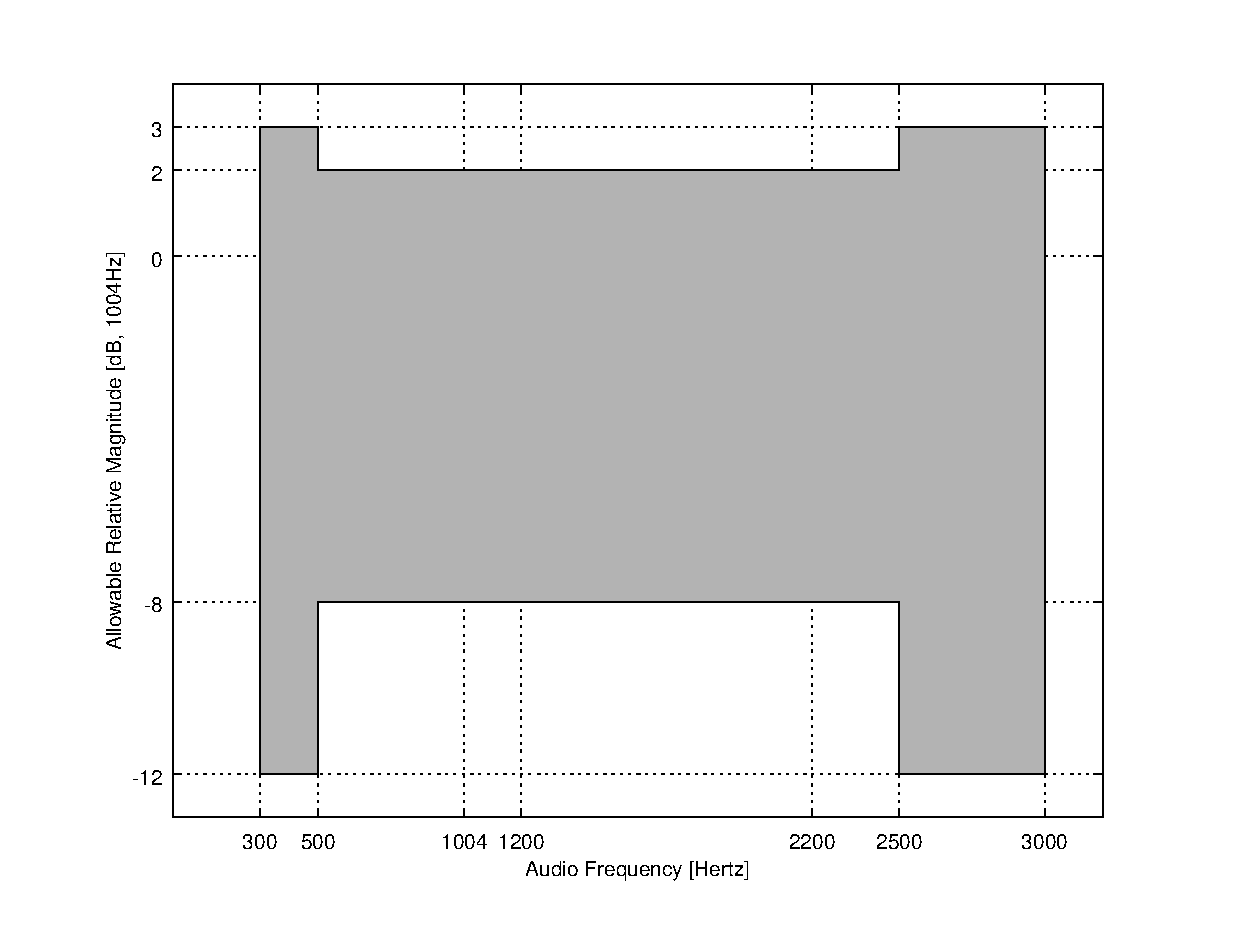
\includegraphics[width=0.7\textwidth]{src/octave/3002}
	\caption{Allowable distortion in a basic 3002 telephone channel}
	\label{fig:3002}
\end{figure}


\section{Carrier Sense Multiple Access}
\label{sec:bell202csma}

Since amateur Bell 202 is a half duplex modulation using repurposed 
FM voice transceivers, 
one of the challenges to packet radio is avoiding multiple stations
transmitting on the same channel at once. 
Other derivatives of ALOHAnet, 
such as the original half duplex 10Mbps Ethernet, 
enjoy the advantage that transmitters can
at least sense when a collision has taken place 
and use that information to abort the transmission of the rest of the frame.

Besides the degenerate case of ignoring the current channel status completely when 
deciding to transmit a pending frame, there are two major algorithms used for CSMA
in APRS;
DWait and P-persistent.

DWait is a deterministic algorithm where each station is assigned a fixed
``quiet time" after the end of another tranmission before they will begin a locally
pending tranmission. This lends itself well to very carefully designed networks
where the relative priority of each station is known and a corresponding DWait time
is set for each station where a shorter DWait will always gain the channel over a longer
one. The requirement for the network to have an overarching design doesn't lend itself
well to the national APRS network, but could be applied effectively for localized 
portions of the APRS network and for ``insular" networks built for special events or
private groups of amateurs.

P-persistent is a stochastic algorithm with two variables: the slot time, and the
probability that a station should transmit at the beginning of a slot. The slot time
should be set to as short of a time interval as possible during which a station can
reliabily identify another station as transmitting 
before beginning its own transmission.
The P value should be tuned based on how likely another station is to transmit 
considering the number of other stations with 
pending traffic attempting to gain the channel.

TODO: Typical settings

\section{Conclusion}


By most measures, Bell 202 is a very poor performing modulation to
be used by amateurs for packet operations. 
One bit symbols cause Bell 202 to suffer from poor spectral efficiency,
HDLC lacks any error correcting codes so single bit errors cause entire 
frames to be droped, and 1200 bits per second is an almost laughably slow
data rate when consumer radio systems are operating in the hundreds of millions
of bits per second.

One property of Bell 202 that is appealing, other than the 
huge legacy systems still using it, is it's relative simplicity.
The fact that amateurs are able to implement Bell 202 modems on
systems as minimalistic as 8 bit microcontrollers and these modems can 
interface with standard voice radios without requiring internal modification 
makes Bell 202 much more accessible than more sophisticated modulations.

Faster data rates and more sophisticated modems should never be discouraged,
but the value of being able to learn about amateur digital communications 
via the simplicity of Bell 202 can't be discounted.
Unfortunately, as the technological landscape where 
protocols such as Bell 202 or AX.25 were developed in moves further into the past,
the need to write additional documentation that gives sufficient context to 
the next generation of packet radio operators is going to become increasingly 
critical to this aspect of the amateur radio hobby.


TODO: Sort citations

\begin{thebibliography}{99}

	\bibitem{millerinterview}
		S. Miller. Personal interview. 25 Mar. 2014.

	\bibitem{ax25spec}
		W. Beech, et al.,
		\emph{AX.25 Link Access Protocol for Amateur Packet Radio Version 2.2}.
		Tucson, Arizona: Tucson Amateur Packet Radio Corp, 1998. 
		\url{http://www.tapr.org/pdf/AX25.2.2.pdf}

	\bibitem{iso13239}
		\emph{Information technoloy --- Telecommunications and information
			exchange between systems --- High-level data link control (HDCL)
		procedures}, ISO Standard 13239, 2002.

	\bibitem{202tspec}
		American Telephone and Telegraph Company,
		\emph{Data Sets 202S and 202T Interface Specification},
		AT\&T Publication 41212,
		July, 1976.

	\bibitem{n1vgphy}
		S. Miller,
		``1200 Baud Packet Radio Details."
		\url{http://n1vg.net/packet/index.php}

	\bibitem{aprsunveiled}
		B. Simmons,
		``APRS Unveiled," in \emph{QEX},
		pp.~19-23,
		Nov./Dec. 2012.

	\bibitem{ituv42}
		\emph{Error-correcting procedures for DCEs using 
		asynchronous-to-synchronous converion}, ITU-T standard V.42, 2002.

	\bibitem{n8urdev}
		J. Ackermann,
		``Setting Your TNC's Audio Drive Level."
		\url{http://www.febo.com/packet/layer-one/transmit.html}

	\bibitem{pattersoninterview}
		R. Patterson. Personal interview. 31 Mar. 2014.

	\bibitem{gatewaypacket}
		S. Horzepa,
		\emph{Your Gateway to Packet Radio},
		Newington, Connecticut: American Radio Relay League, 1989.

\end{thebibliography}


\end{document}

